\chapter{数值模拟}

在过去的章节中,我们介绍了量子线路的基本概念,并介绍了如何使用基于Pauli路径积分的模拟算法来模拟量子线路。并在一些具体的线路模型中,研究了模拟算法的计算复杂度和误差。特别地,发现了在一些情况下,比如含噪声的变分量子线路,算法的计算复杂度关于线路规模是多项式关系。
虽然,我们定性地分析了模拟算法的计算复杂度,但是我们还没有给出具体的数值模拟结果。多项式复杂度对于实际的模拟算法来说是一个很好的性质,但是是否实用还有待进一步的数值模拟结果的验证。
例如,在定理~\ref{thm:main}中,我们得到了对于噪声\textbf{情况1}时,算法的计算复杂度是:
\begin{equation*}
    \mathrm{Poly}(n) \order{L} \bigg(\frac{\norm{O}_\infty}{\varepsilon \sqrt{\delta}} \bigg)^{\order{\frac{1}{\gamma}}},
\end{equation*}
其中$n$是线路的规模,$L$是线路的深度,$\varepsilon$是算法的精度,$\delta$是算法失败的概率,$\gamma=\min\{p|{p \in \{p_x,p_y,p_z\},p\neq 0}\}$是噪声率,$\norm{O}_\infty$是可观测量的无穷范数。当噪声强度$\gamma$很小时,例如$\gamma=0.01$,我们可以得到算法的计算复杂度是$\mathrm{Poly}(n) \order{L} \bigg(\frac{\norm{O}_\infty}{\varepsilon \sqrt{\delta}} \bigg)^{{100}}$,这是一个难以实现的计算复杂度。万幸的是,实际情况下的计算复杂度并不会达到这么高的程度,我们将在本章中具体说明。

除此之外,在这一章中,我们将使用基于Pauli路径积分的模拟算法来模拟一些量子线路的具体实例。并与实际的实验结果进行比较,以验证模拟算法的有效性。

在本章中,如未加说明,我们将假设环境噪声处于\textbf{情况1},这是因为在实际的量子计算机中,很难出现纯净的单独类型的Pauli错误。因此假设$p_x\neq 0,p_y\neq 0,p_z\neq 0$是合理的,此时与噪声关联的Hamming Weight 根据式~\eqref{eq:noise_hamming_weight}可以得到:
\begin{equation*}
    \abs{\bm{s}}_{\mathcal{N}}=\abs{\bm{s}}_X + \abs{\bm{s}}_Y + \abs{\bm{s}}_Z.
\end{equation*}
在这种情况下,正是原始的Hamming Weight定义,为了方便,我们将在本章中使用$\abs{\bm{s}}$来表示。


\section{模拟算法的计算复杂度分析}
对于变分量子线路,根据式~\eqref{eq:vqa:cost},在噪声\textbf{情况1}下,模拟算法的计算复杂度是:
\begin{equation*}
    \mathrm{Poly}(n) \order{L}2^M,
\end{equation*}
其中$n$是线路的规模,$L$是线路的深度,$M$是截断变量。可以看到在过去理论估计中,计算复杂度关于截断变量$M$是指数关系。这个指数因子的来源是由于在Pauli 路径枚举过程中,根据式~\eqref{eq:vqa:case1:N_M},符合条件$\abs{\bm{s}}\leq M$的Pauli路径数目是指数级别的。在这一节中,我们将通过具体的数值模拟结果来估计,给定截断变量$M$时,满足条件Pauli路径的真实数目。


对于截断变量的取值,根据引理~\ref{lemma:MSE_l}的注释,我们可以得到
对于变分量子线路在退极化噪声下,如果式~\eqref{eq:E_cross_equals_0}成立,那么对任意的$\nu > 0$,只要截断参数$M$满足:
\begin{equation}\label{eq:depolarizing_M}
    M\geq\frac{1}{2\lambda}\ln{\frac{\norm{O}_\infty^2}{\nu}},
\end{equation}
其中$\lambda$是退极化噪声的强度,那么含噪声期望值模拟的均方误差满足:
\begin{equation}
    \mathbb{E}_{\bm{\theta}}\left[\left(\widetilde{\langle O\rangle}-\widehat{\langle O\rangle}\right)^2\right]\leq\nu.
\end{equation}
事实上,在实际计算中,$M$也并不需要取到这么大的值,我们将在本节中具体用数值说明。

\subsection{计算复杂度与截断变量$M$的关系}

因为截断Pauli路径模拟算法的计算复杂度主要来自于具有非平凡贡献的Pauli路径的数量,因此我们将通过计算具有非零贡献的Pauli路径的数量来估计模拟算法的计算复杂度。在这一节中,我们将通过具体的数值模拟结果来估计,给定截断变量$M$时,满足条件Pauli路径的真实数目。


\begin{figure}[htbp]
    \centering
    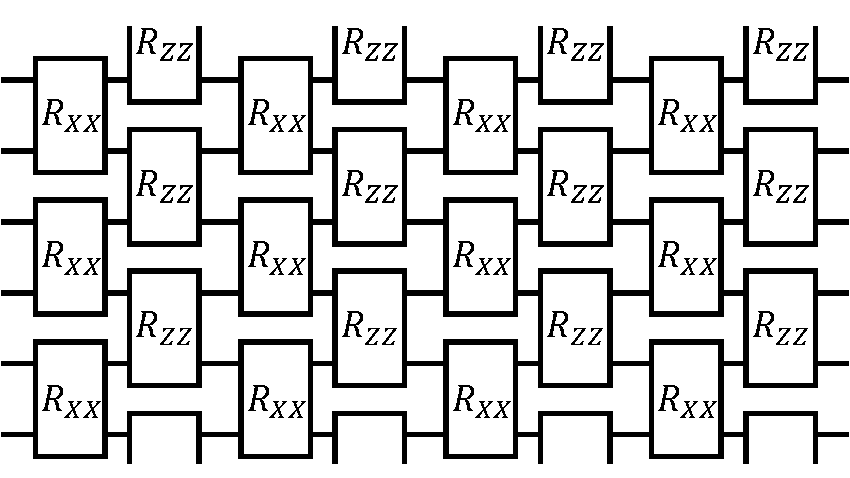
\includegraphics[width=0.5\textwidth]{figures/XX_ZZ_Ansatz.pdf}
    \caption{数值模拟计算复杂度与$M$的关系中使用的量子线路示意图}\label{fig:XX_ZZ_Ansatz}
\end{figure}

在我们的模拟中,我们考虑了一个具体的MaxCut问题实例。
对于给定的量子比特数$n$,我们随机生成一个$n\times n$的邻接$(0,1)$矩阵$A$,其中每个元素为$1$的概率为$0.5$。
可观测量$O$基于MaxCut问题构建,并按照给出的邻接矩阵$A$构造:
\begin{equation}
    O=\sum_{A_{i,j}=1} Z_iZ_j.
\end{equation}
在模拟中,初始状态的密度矩阵设为$\rho=\ketbra{0}{0}^{\otimes n}$。
考虑的量子线路$\mathcal{U}$如图~\ref{fig:XX_ZZ_Ansatz}所示,该线路由交替的$R_{XX}$和$R_{ZZ}$ 旋转门组成,其中第一个量子比特上的不完整$R_{ZZ}$门表示它们作用于第一个和最后一个量子比特。


\begin{figure}[hbp]
    \centering
    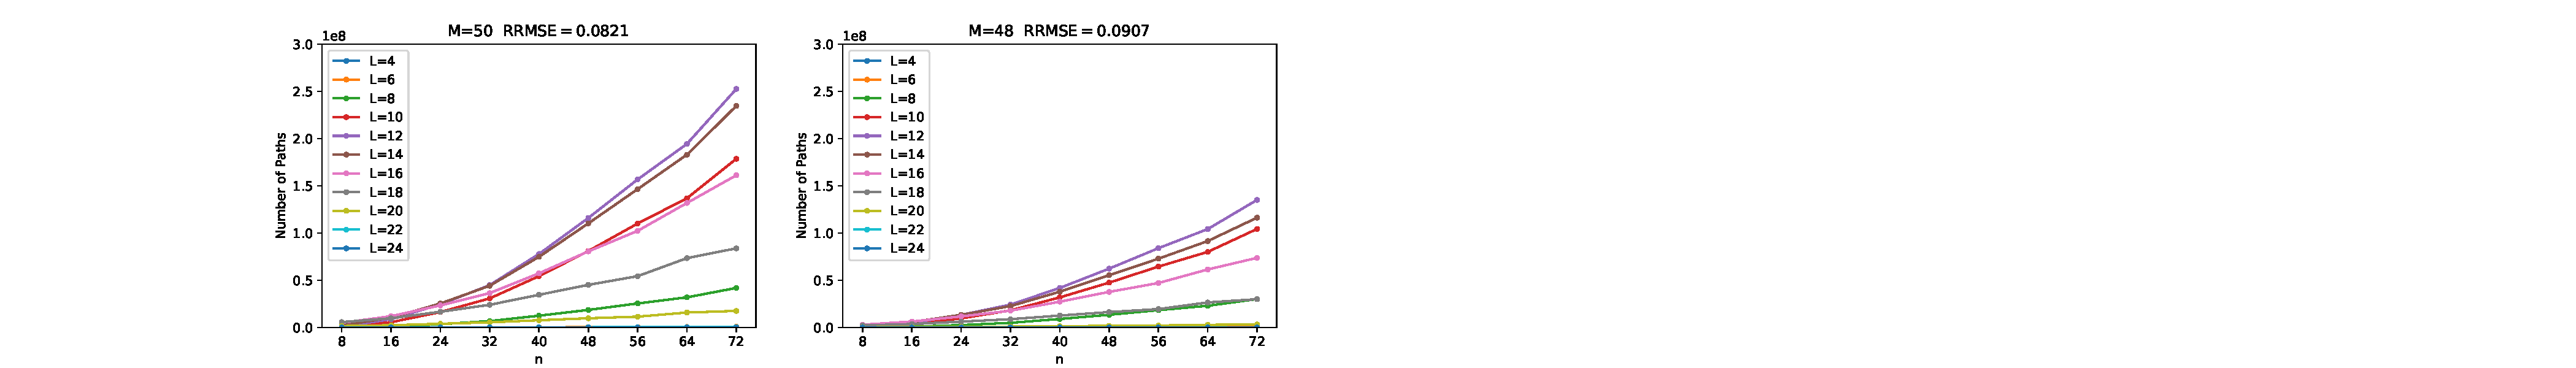
\includegraphics[width=\textwidth]{figures/depth_path2_p1}
    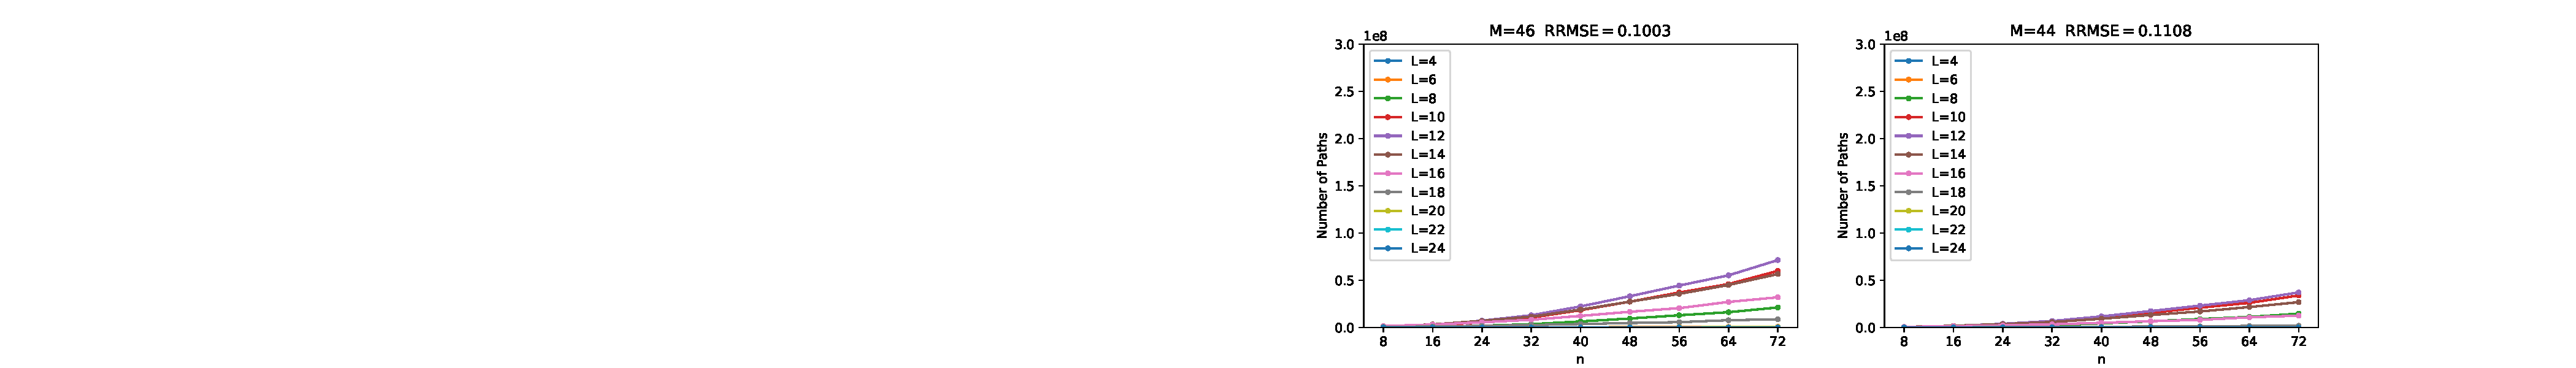
\includegraphics[width=\textwidth]{figures/depth_path2_p2}
    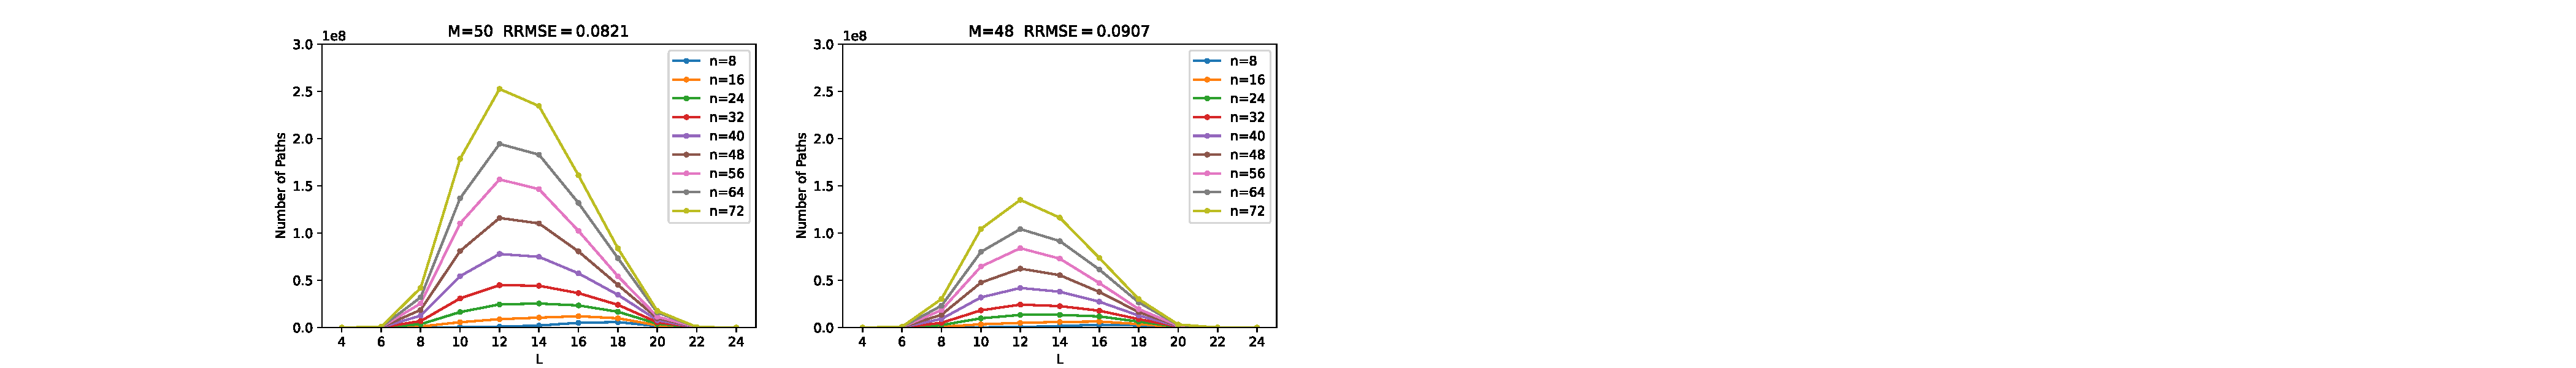
\includegraphics[width=\textwidth]{figures/depth_path_p1}
    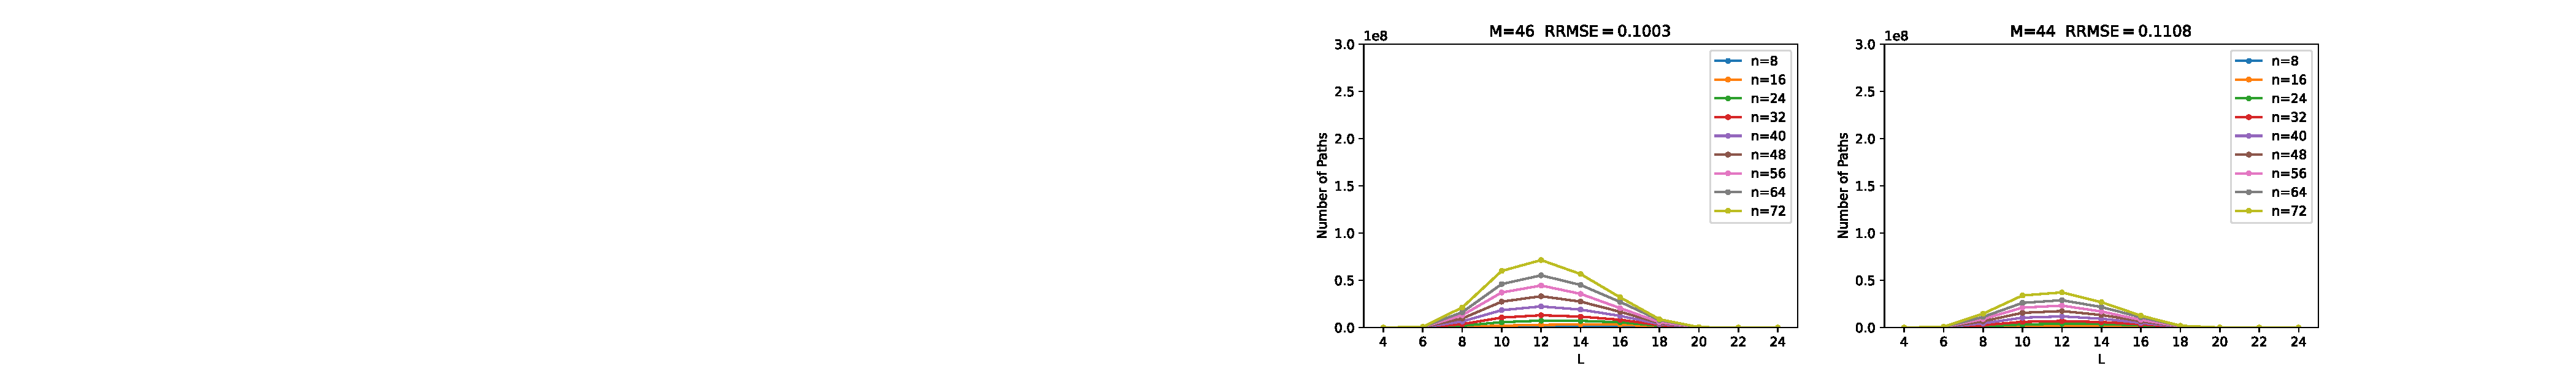
\includegraphics[width=\textwidth]{figures/depth_path_p2}
    \caption{具有非零贡献且$\abs{\bm{s}}\leq M$的Pauli路径$\bm{s}$的数量}\label{fig:numerical_cost}
\end{figure}

根据式~\eqref{eq:depolarizing_M},对于固定的量子线路,不同的截断参数$M$对应于在固定噪声率下由$\frac{\sqrt{\mathbb{E}_{\bm{\theta}}\abs{\widetilde{\langle O \rangle}-\widehat{\langle O \rangle}}^2}}{\norm{O}_\infty}$给出的相对均方根误差界(Relative Root Mean Square Error,RRMSE)。

对于不同的量子比特数$n$和线路的深度$L$,我们计算了权重$\abs{s}\leq M$且具有非零贡献的Pauli路径$s$的数量,结果如图~\ref{fig:numerical_cost}所示。前两行的每个图显示了在固定$M$的情况下,随着$n$的增加,具有非零贡献的Pauli路径的数量的变化。可以看到,在固定$M$的情况下,随着$n$的增加,对所有不同深度$L$的情况,具有非零贡献的Pauli路径的数量将适度增加,并显著小于理论分析的上界$\mathrm{Poly}(n)2^M$。


后两行的每个图显示了在固定$M$的情况下,随着$L$的增加,具有非零贡献的Pauli路径的数量的变化。我们观察到,对于给定的RRMSE界,路径数量先增加然后随着$L$的增加而减少。
这意味着,在给定精度下模拟含噪声量子线路的计算复杂度随着线路深度的增加呈现出先增加后减少的趋势。这与文献~\cite{noh2020efficient}中的发现一致。
其中的RRMSE界是由式~\eqref{eq:depolarizing_M}在噪声率$\lambda=0.2$下给出的。


另一方面,通过式~\ref{eq:depolarizing_M},可以看到不同的截断参数$M$在给定的RRMSE界下也对应了一个具体的噪声强度$\lambda$。
假设,RRMSE界固定为$0.0821$,按图中给出的数据将$M$取值为$M=50,48,46,44$,此时对应的噪声强度为$\lambda=0.2,0.21,0.22,0.23$(两位有效数字)。
从数值结果中可以看到,对于不同的$M$,在给定线路规模$n$和深度$L$的情况下,具有非零贡献的Pauli路径的数量是不同的。这说明在实际的模拟中,噪声的大小将会显著影响模拟算法的计算复杂度。


\subsection{模拟误差与截断变量$M$的关系}


\section{Ising模型演化}